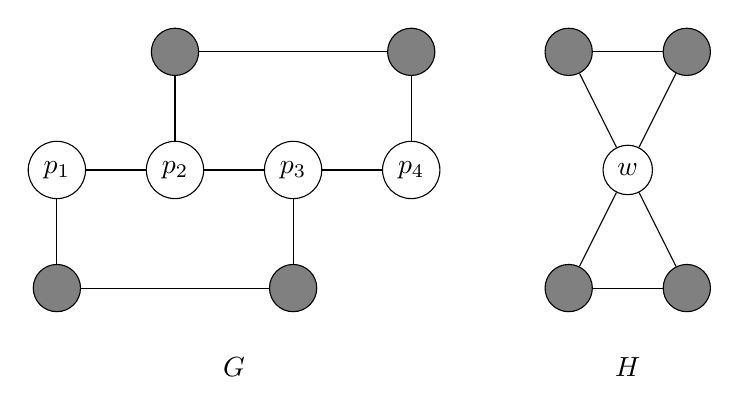
\begin{tikzpicture}

\node [circle, minimum height=0.6cm, draw] (v1) at (0,0) {$p_1$};
\node [circle, minimum height=0.6cm, draw] (v2) at (1.5,0) {$p_2$};
\node [circle, minimum height=0.6cm, draw] (v3) at (3,0) {$p_3$};
\node [circle, minimum height=0.6cm, draw] (v4) at (4.5,0) {$p_4$};
\node [circle, minimum height=0.6cm, draw, fill=gray] (v6) at (1.5,1.5) {};
\node [circle, minimum height=0.6cm, draw, fill=gray] (v5) at (4.5,1.5) {};
\node [circle, minimum height=0.6cm, draw, fill=gray] (v7) at (0,-1.5) {};
\node [circle, minimum height=0.6cm, draw, fill=gray] (v8) at (3,-1.5) {};
\draw  (v1) edge (v2);
\draw  (v2) edge (v3);
\draw  (v3) edge (v4);
\draw  (v4) edge (v5);
\draw  (v5) edge (v6);
\draw  (v6) edge (v2);
\draw  (v1) edge (v7);
\draw  (v7) edge (v8);
\draw  (v8) edge (v3);


\node [circle, minimum height=0.6cm, draw, fill=gray] (v9) at (6.5,1.5) {};
\node [circle, minimum height=0.6cm, draw, fill=gray] (v10) at (8,1.5) {};
\node [circle, minimum height=0.6cm, draw] (v11) at (7.25,0) {$w$};
\node [circle, minimum height=0.6cm, draw, fill=gray] (v13) at (6.5,-1.5) {};
\node [circle, minimum height=0.6cm, draw, fill=gray] (v12) at (8,-1.5) {};
\draw  (v9) edge (v10);
\draw  (v10) edge (v11);
\draw  (v11) edge (v9);
\draw  (v11) edge (v12);
\draw  (v12) edge (v13);
\draw  (v13) edge (v11);


\node at (2.25,-2.5) {$G$};
\node at (7.25,-2.5) {$H$};
\end{tikzpicture}